\chapter{Terceiro Projeto: Sistema para Venda de Produtos}\label{cap:terceiroProjeto}
\epigraph{``\textit{A imaginação é mais importante que o conhecimento}''.}{Albert Einstein}

\lettrine[lines=4, lhang=0.1, lraise=0, loversize=0.2, findent=0.1em]{\textcolor{corAzulTema}{N}}{ESTE} Capítulo iremos construir mais um projeto completo, concluindo os conhecimentos básicos para que você possa construir praticamente qualquer tipo de sistema que lide com banco de dados, ou seja, aprenderemos a lidar com a implementação de cadastros que têm relacionamentos ``muitos para muitos''.


\section{Introdução}

Finalmente estamos aptos a construir uma aplicação Web em Java com a maioria das funcionalidades necessárias à maioria das aplicações Web que você desenvolverá na sua vida profissional. Iremos incrementar a aplicação criada no Capítulo~\ref{cap:primeiroProjeto} criando mais alguns cadastros e amarrando todos eles em um cadastro de vendas de produtos. Vamos lá!

Além de clientes, cidades e estados, criaremos mais três cadastros com inserção, alteração e remoção de registros: unidade de medida, produto e fornecedor. Com esses seis cadastros desenvolveremos a interface gráfica das vendas, onde poderemos gerar novas vendas e, após serem feitas, será permitido que sejam canceladas.

Na Figura~\ref{fig:cap08ModeloFisico} pode ser visto o modelo físico da base de dados \texttt{venda\_produtos}. Note que o nome da base é diferente do projeto anterior. Para esse projeto não disponibilizarei o script SQL para a criação da base de dados pois, além da estrutura, teremos algumas inserções já prontas para podermos testar. Para gerar a base, com o MariaDB/MySQL em execução, abra o modelo da base no MySQL Workbench, disponibilizado nos arquivos do projeto. Com o modelo aberto, clique no menu \destaque{\textit{Database}} e na opção \destaque{\textit{Forward Engineer...}} e siga o assistente. A base de dados, as tabelas, e os relacionamentos serão criados e várias inserções para as tabelas estado, cidade, cliente, fornecedor, unidade\_medida e produto.

\FloatBarrier
\begin{figure}[!htbp]
    \centering
    \caption{Diagrama do modelo físico da base de dados}
    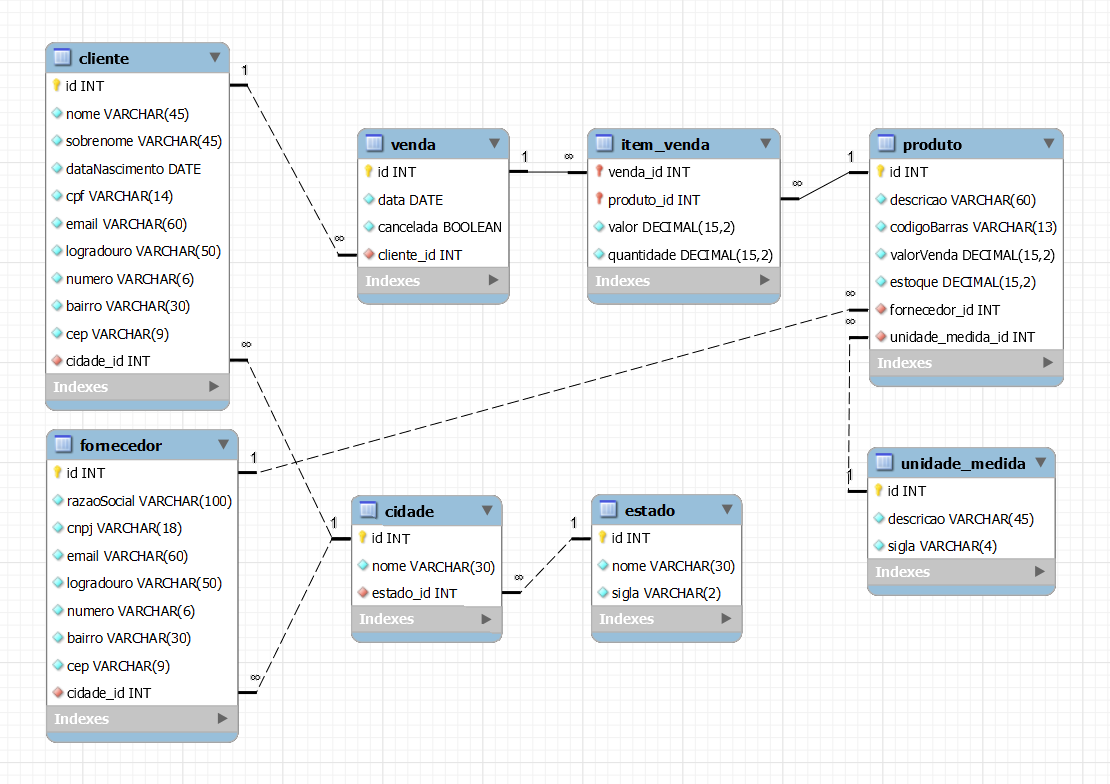
\includegraphics[scale=0.5]{imagens/cap08ModeloFisico}
    \\\textbf{Fonte:} Elaborada pelo autor
    \label{fig:cap08ModeloFisico}
\end{figure}
\FloatBarrier

O diagrama de classes do projeto pode ser visto Figura~\ref{fig:cap08DiagramaClasses}. Veja que a classe \texttt{ItemVenda} é a classe que fará o papel de viabilizar o relacionamento muitos-para-muitos entre produtos e vendas.

\FloatBarrier
\begin{figure}[!htbp]
    \centering
    \caption{Diagrama de classes das entidades}
    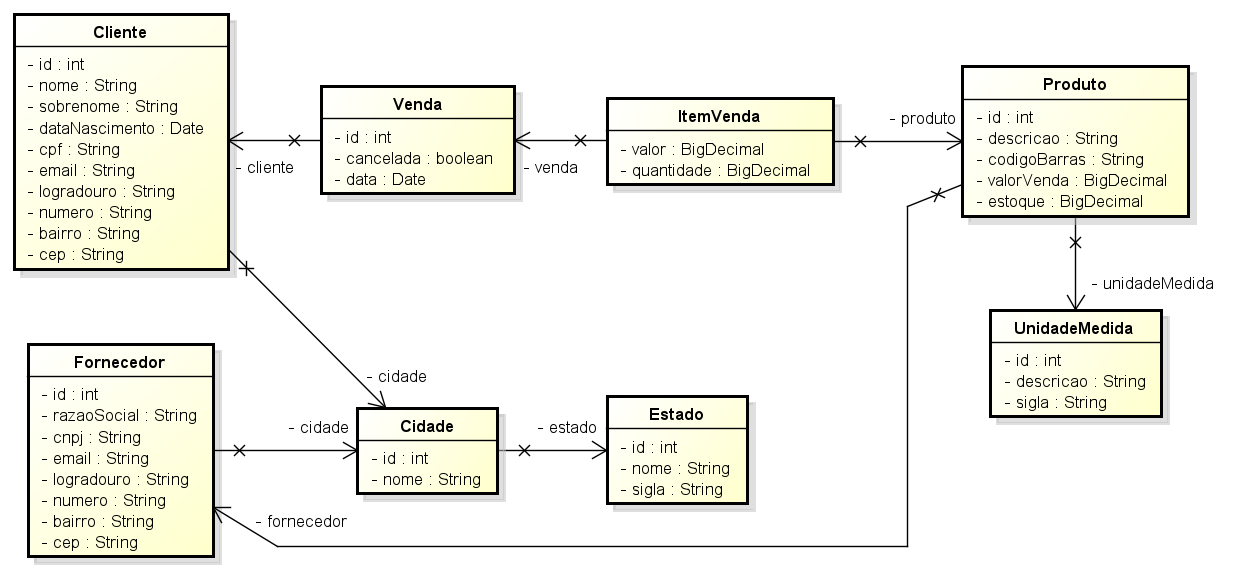
\includegraphics[scale=0.45]{imagens/cap08DiagramaClasses}
    \\\textbf{Fonte:} Elaborada pelo autor
    \label{fig:cap08DiagramaClasses}
\end{figure}
\FloatBarrier

Para que esse Capítulo não fique gigantesco, irei focar apenas nas novidades ou modificações que foram feitas em relação ao projeto anterior. Você poderá pegar o projeto pronto. A entidade \texttt{Produto} será usada como base para entendermos o que foi alterado e depois toda a parte da venda propriamente dita será detalhada com mais afinco.


\section{Construindo o Sistema}

Esta seção será dividida em várias subseções para que possamos organizar o que foi modificado em relação ao sistema anterior além, é claro, das funcionalidades novas. Os seis cadastros base são similares, então apenas um, como já explicado, será detalhado e o restante é por sua conta dar uma olhada, bastando consultar o código pronto no projeto disponibilizado.


\subsection{Entidades e Validações}

Começaremos discutindo nossas entidades. Todos os membros de todas elas agora serão de tipos de referência, ou seja, qualquer tipo que não seja primitivo. O tipo \inlineJavaCode{int} que usamos para definir os identificadores delas, agora passarão a ser do tipo \texttt{Long}. Todos os tipos numéricos decimais serão do tipo \texttt{BigDecimal}, principalmente quando precisarmos representar valores monetários, fugindo assim da imprecisão dos tipos de ponto flutuante, pois dinheiro é algo muito importante e precisamos tomar muito, muito, MUITO cuidado com esse tipo de dado em um sistema de verdade. Além disso, cada atributo será anotado com pelo menos uma anotação de validação, pois todos os nossos objetos das entidades serão validados, obrigatoriamente antes de serem submetidos aos seus respectivos DAOs, filtrando possíveis tentativas de adulteração dos dados submetidos através dos formulários. Na entidade \texttt{Produto}, apresentada na Listagem~\thechapter.\ref{listagem:projetos/capitulo08/VendaProdutos/src/java/vendaprodutos/entidades/Produto.java}, podemos ver isso.

\javaCode{Entidade ``Produto''\newline%
Arquivo: \texttt{vendaprodutos/entidades/Produto.java}}{projetos/capitulo08/VendaProdutos/src/java/vendaprodutos/entidades/Produto.java}

Sempre precedendo a definição de um atributo da classe utilizaremos essas anotações. Na linha 17 o atributo identificador da entidade \texttt{Produto} é declarado e, logo antes, na linha 16, é usada a anotação \inlineJavaCode{@NotNull} que indica que um objeto do tipo \texttt{Produto}, ao ser validado, não poderá ter esse atributo configurado com \inlineJavaCode{null}. Veremos o mecanismo de validação já já. O atributo \texttt{descricao} é anotado com \inlineJavaCode{@NotNull}, que já aprendemos, e \inlineJavaCode{@Size} que dependendo do tipo, verificará o tamanho do valor do mesmo. Para \texttt{Strings}, que é o nosso caso, é a quantidade de caracteres. Na linha 20 temos então que a descrição dos produtos pode ter no mínimo um caracetere e no máximo 60. Note que todas as nossas validações serão consistentes com as restrições existentes no modelo físico do banco de dados. O código de barras de um produto terá obrigatoriamente que bater com um padrão de 13 dígitos, usando para isso a anotação \inlineJavaCode{@Pattern} com o atributo \texttt{regexp} (\textit{regular expression}). Essa expressão regular diz que o padrão deve casar com a String inteira, sendo que isso é indicado pelos meta-símbolos \^{} e \$ que significam, respectivamente, início e fim da \texttt{String}. O méta-símbolo \textbackslash{}d significa um dígito ($0$ a $9$) e há a necessidade de se usar duas contrabarras, pois como em Java a contrabarra indica um caracetere de escape, precisamos usar duas para escapá-la. O atributo \texttt{message} de \inlineJavaCode{@Pattern} é usado para criarmos uma mensagem personalizada para quando o produto for validado e esse atributo estiver fora do que é esperado.

A anotação \inlineJavaCode{@PositiveOrZero} indica que o atributo do tipo BigDecimal deve ser, zero ou qualquer valor positivo. As outras anotações que usaremos nas outras entidades são \inlineJavaCode{@Positive} para valores positivos obrigatoriamente (zero não é positivo nem negativo!) e \inlineJavaCode{@Email} para verificar se o valor representa um formato válido de e-mail. A implementação de referência da \textit{Jakarta Bean Validation} faz parte do Jakarta EE 8, que estamos usando, e é fornecida pelo Hibernate Validator.

\begin{saibaMais}
    O site oficial da especificação e da implementação da API \textit{Bean Validation} pode ser acessada pelo link \url{https://beanvalidation.org/}
\end{saibaMais}

A validação dos objetos será feita sempre nos Servlets e é implementada pelo método \inlineJavaCode{validar}, que tem sua implementação iniciada na linha 150 da classe \texttt{Utils}, mostrada na Listagem~\thechapter.\ref{listagem:projetos/capitulo08/VendaProdutos/src/java/vendaprodutos/utils/Utils.java}.

\javaCode{Classe ``Utils'' com métodos estáticos utilitários\newline%
Arquivo: \texttt{vendaprodutos/utils/Utils.java}}{projetos/capitulo08/VendaProdutos/src/java/vendaprodutos/utils/Utils.java}

Na nossa implementação da validação de objetos forneceremos a opção do usuário do método ignorar a validação de atributos de uma classe, caso seja necessário. Por exemplo, um \texttt{Produto} novo não terá identificador até que seja persistido, mas precisaremos validá-lo antes de ser enviado ao seu DAO. O método validar faz uso do método estático privado \inlineJavaCode{validarObj} que é quem invoca de fato a infraestrutura de validação. Veja o código, está todo comentado. O método \inlineJavaCode{validar} lançará uma exceção do tipo SQLException caso o objeto seja inválido e essa exceção terá encapsulada como mensagem que conterá todas as inconsistências identificadas no objeto. Essa mensagem será configurada com uma série de \textit{tags} \inlineHTMLCode{<li>} e será usada na página de erros. Veremos essa questão da página de erros mais adiante no Capítulo.

Vamos ver agora o que mudou na nossa camada de persistência.


\subsection{DAO}

Temos duas novidades na nossa camada de persistência. A primeira é a implementação da interface \texttt{AutoCloseable} que permitirá que usemos objetos dos nossos DAOs na construção \textit{try-with-resources} que, por sua vez, fará o fechamento automático da conexão dos DAOs ao terminarem de serem utilizados. Para isso precisaremos implementar o método \inlineJavaCode{close} que substituirá o nosso antigo \inlineJavaCode{fecharConexao}. A implementação do DAO genérico é mostrada na Listagem~\thechapter.\ref{listagem:projetos/capitulo08/VendaProdutos/src/java/vendaprodutos/dao/DAO.java}, sendo que o método \inlineJavaCode{close} pode ser visto a partir da linha 57.

\javaCode{DAO genérico\newline%
Arquivo: \texttt{vendaprodutos/dao/DAO.java}}{projetos/capitulo08/VendaProdutos/src/java/vendaprodutos/dao/DAO.java}

A outra mudança que temos em nossos DAOs é que agora toda entidade ao ser persistida, será modificada para conter o identificador que foi gerado pelo SGBD. Na a Listagem~\thechapter.\ref{listagem:projetos/capitulo08/VendaProdutos/src/java/vendaprodutos/dao/ProdutoDAO.java} onde é apresentado o DAO para produtos.

\javaCode{Código da classe ``ProdutoDAO''\newline%
Arquivo: \texttt{vendaprodutos/dao/ProdutoDAO.java}}{projetos/capitulo08/VendaProdutos/src/java/vendaprodutos/dao/ProdutoDAO.java}

Veja que a criação do \texttt{PreparedStatement} do método \inlineJavaCode{salvar} agora usa outra versão do método \inlineJavaCode{prepareStatement(...)} de \texttt{Connection}. Nessa versão, além da String contendo o código SQL que será executado, é passado um array de Strings com o nome da ou das colunas que representam as chaves primárias daquela tabela. Essa ``artimanha'' funciona para colunas que são auto incrementáveis, que é o caso dos nossos identificadores. Precisaremos dessa característica no cadastro das vendas. Veremos isso mais para frente. Quando fazemos uso desse recurso, após a persistência do objeto, que gerará uma nova linha/registro/tupla na tabela, precisaremos usar o mesmo \texttt{PreparedStatement} para obter a ou as chaves. Isso será feito no método \inlineJavaCode{getChavePrimariaAposInsercao(...)} da classe \texttt{Utils} (linha 96 da Listagem~\thechapter.\ref{listagem:projetos/capitulo08/VendaProdutos/src/java/vendaprodutos/utils/Utils.java}). Como consistentemente estamos usando uma coluna chamada \texttt{id} como chave primária auto incrementável, usaremos esse método para todas as nossas entidades, com exceção da \texttt{ItemVenda} que funcionará de outra forma.

Muito bem, temos nossas entidades prontas para serem validadas e a camada de persistência atualizada. Vamos ver agora o que mudou nos nossos Servlets.


\subsection{Servlets}

Falar do produto, pois tem BigDecimal. ProdutoServlet.
Falar dos métodos que retornam null na classe Utils caso o dado venha inválido do formulário.

Listagem~\thechapter.\ref{listagem:projetos/capitulo08/VendaProdutos/src/java/vendaprodutos/controladores/ProdutosServlet.java}.

\javaCode{Código-fonte do Servlet ``ProdutosServlet''\newline%
Arquivo: \texttt{vendaprodutos/controladores/ProdutosServlet.java}}{projetos/capitulo08/VendaProdutos/src/java/vendaprodutos/controladores/ProdutosServlet.java}

\subsection{Tratamento de Erros}

Mostrar página de tratamento de erros.

Listagem~\thechapter.\ref{listagem:projetos/capitulo08/VendaProdutos/web/erro.jsp}.

\htmlCode{Página para exibição de erros\newline%
Arquivo: \texttt{/erro.jsp}}{projetos/capitulo08/VendaProdutos/web/erro.jsp}


\subsection{Cadastro de Vendas}

Falar das entidades e dos DAOs.

Venda

Listagem~\thechapter.\ref{listagem:projetos/capitulo08/VendaProdutos/src/java/vendaprodutos/entidades/Venda.java}.

\javaCode{Entidade ``Venda''\newline%
Arquivo: \texttt{vendaprodutos/entidades/Venda.java}}{projetos/capitulo08/VendaProdutos/src/java/vendaprodutos/entidades/Venda.java}

ItemVenda

Listagem~\thechapter.\ref{listagem:projetos/capitulo08/VendaProdutos/src/java/vendaprodutos/entidades/ItemVenda.java}.

\javaCode{Entidade ``ItemVenda''\newline%
Arquivo: \texttt{vendaprodutos/entidades/ItemVenda.java}}{projetos/capitulo08/VendaProdutos/src/java/vendaprodutos/entidades/ItemVenda.java}


VendaDAO

Listagem~\thechapter.\ref{listagem:projetos/capitulo08/VendaProdutos/src/java/vendaprodutos/dao/VendaDAO.java}.

\javaCode{Código da classe ``VendaDAO''\newline%
Arquivo: \texttt{vendaprodutos/dao/VendaDAO.java}}{projetos/capitulo08/VendaProdutos/src/java/vendaprodutos/dao/VendaDAO.java}

ItemVendaDAO

Listagem~\thechapter.\ref{listagem:projetos/capitulo08/VendaProdutos/src/java/vendaprodutos/dao/ItemVendaDAO.java}.

\javaCode{Código da classe ``ItemVendaDAO''\newline%
Arquivo: \texttt{vendaprodutos/dao/ItemVendaDAO.java}}{projetos/capitulo08/VendaProdutos/src/java/vendaprodutos/dao/ItemVendaDAO.java}

Falar do Servlet e da atualização do estoque. Falar do cancelamento da venda.

Listagem~\thechapter.\ref{listagem:projetos/capitulo08/VendaProdutos/src/java/vendaprodutos/controladores/VendasServlet.java}.

\javaCode{Código-fonte do Servlet ``VendasServlet''\newline%
Arquivo: \texttt{vendaprodutos/controladores/VendasServlet.java}}{projetos/capitulo08/VendaProdutos/src/java/vendaprodutos/controladores/VendasServlet.java}

Páginas

Listagem~\thechapter.\ref{listagem:projetos/capitulo08/VendaProdutos/web/formularios/vendas/listagem.jsp}.

\htmlCode{Código da listagem de Vendas\newline%
Arquivo: \texttt{/formularios/vendas/listagem.jsp}}{projetos/capitulo08/VendaProdutos/web/formularios/vendas/listagem.jsp}


Listagem~\thechapter.\ref{listagem:projetos/capitulo08/VendaProdutos/web/js/formularios/vendas/listagem.js}.

\javaScriptCode{\textit{Script} para cancelamento de Vendas\newline%
Arquivo: \texttt{/js/formularios/vendas/listagem.js}}{projetos/capitulo08/VendaProdutos/web/js/formularios/vendas/listagem.js}


Listagem~\thechapter.\ref{listagem:projetos/capitulo08/VendaProdutos/web/formularios/vendas/novo.jsp}.

\htmlCode{Formulário de cadastro de novas Vendas\newline%
Arquivo: \texttt{/formularios/vendas/novo.jsp}}{projetos/capitulo08/VendaProdutos/web/formularios/vendas/novo.jsp}


Listagem~\thechapter.\ref{listagem:projetos/capitulo08/VendaProdutos/web/js/formularios/vendas/novo.js}.

\javaScriptCode{\textit{Script} para tratamento de novas Vendas\newline%
Arquivo: \texttt{/js/formularios/vendas/novo.js}}{projetos/capitulo08/VendaProdutos/web/js/formularios/vendas/novo.js}


\section{Resumo}

Neste Capítulo construímos uma aplicação Web completa para a venda de produtos. Utilizamos para isso tudo que aprendemos até agora. Com isso você já é capaz de implementar a maioria dos tipos de cadastros que aparecerão em sistemas do mundo real. Parabéns! No próximo Capítulo vai ser a sua vez de fazer tudo do zero, reescrevendo e melhorando o sistema de locação de DVDs. 


\section{Projetos}

\begin{projetoSemArquivo}{}{}{}
    Modifique a implementação do projeto desenvolvido neste Capítulo para permitir que em uma venda possa existir mais de um item de venda igual. Na implementação atual isso não é permitido, pois cada registro da tabela \texttt{item\_venda} tem como chave primária a composição das duas chaves estrangeiras que a relaciona com as tabelas \texttt{produto} e \texttt{venda}. Será necessário modificar o modelo físico e alguns detalhes da implementação do projeto, tanto do lado do servidor, quanto do lado do cliente.
\end{projetoSemArquivo}
